\documentclass[numbers=noenddot,12pt,a4paper]{scrartcl}
\usepackage[greek,ngerman]{babel}
\usepackage[T1]{fontenc}
\usepackage[utf8]{inputenc}
\usepackage{fullpage}
\usepackage{libertine}
\usepackage{ziffer}
\usepackage{graphicx}
\usepackage{units}
\usepackage[infoshow]{tabularx}
\usepackage{amsmath}
\usepackage{amssymb}
\usepackage{wrapfig}
\usepackage{esint}
\usepackage{float}
\usepackage{wrapfig}
\usepackage[font=small]{caption}
\usepackage{subcaption}
\usepackage{lscape}
\usepackage{hyperref}

\renewcommand{\thefigure}{Abb. \arabic{figure}}

\captionsetup[wrapfigure]{name=}
\captionsetup[figure]{name=}
\newcommand{\degree}{^\circ}
\newcommand{\diff}{\textnormal{d}}
\newcommand{\tenpo}[1]{\cdot 10^{#1}}
\newcommand{\greek}[1]{\greektext#1\latintext}
\newcommand{\ix}[1]{_\text{#1}}
\newcommand{\imag}{\mathbf{i}}

\title{Protokoll: Solarzelle}
\author{Tom Kranz, Philipp Hacker}
\date{\today}

\begin{document}
%\setcounter{page}{2}
%\setcounter{section}{1}
\maketitle
\begin{center}
Betreuer: J. Walowski\\
Versuchsdatum: 4.11.2014/5.11.2014\\
\begin{table}[h]
\centering
Note: %TODO Gute Note erhalten :)
\begin{tabularx}{1.5cm}{|X|}
\hline \\ \\
\hline
\end{tabularx}
\end{table}
\end{center}
\vspace*{\fill}
\tableofcontents
\vfill
\newpage
\section{Einleitung}
Solarzellen sind aktive elektrische Bauelemente zur Umwandlung von Strahlungs- in elektrische Energie. In diesem Versuch sollen die Eigenschaften einer Solarzelle im Betrieb beleuchtet werden -- dazu wird die Strom- und Spannungs-Charakteristik einer handelsüblichen Solarzelle unter verschiedenen Bedingungen aufgenommen und näher ausgewertet. Insbesondere wird dabei auf den Diodencharakter dieses Halbleiterbauelements eingegangen.
\section{Grundlegendes}
Die einfache Solarzelle ist ein Halbleiterbauelement, genauer gesagt: Eine Diode. Als solche benötigt das Verständnis ihrer Funktionsweise Kenntnis von den Eigenschaften von Halbleitern und besonders von p-n-Übergängen.
\subsection{Halbleiter}
\begin{wrapfigure}{r}{0.4\textwidth}
	\vspace{-3em}
	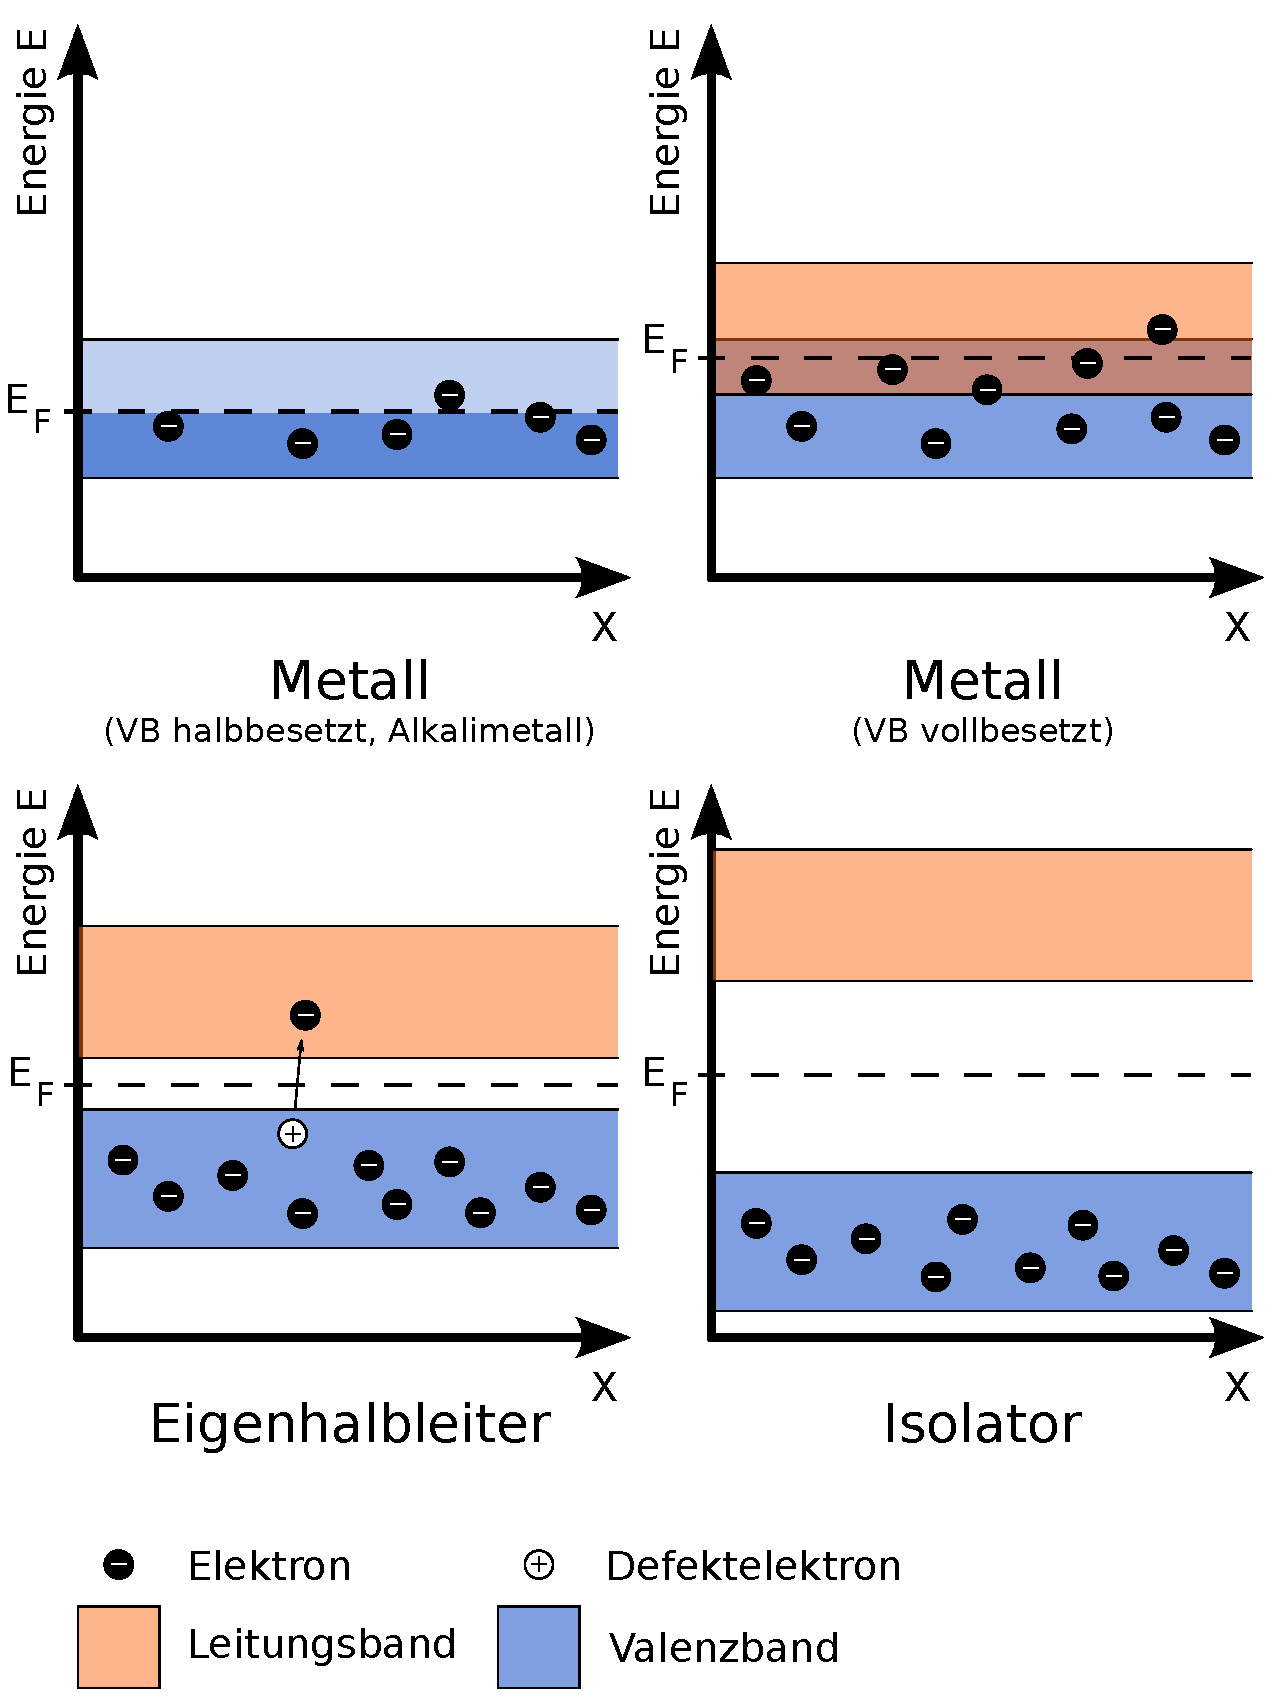
\includegraphics[width=0.4\textwidth]{ebmde.pdf}
	\caption{Schema der Energiebänder in verschiedenen Materialklassen}
	\label{img:Eniv}
\end{wrapfigure}
Halbleiter sind Stoffe, deren elektrische Leitfähigkeit je nach Anwendungsgebiet mehr oder weniger leicht um Größenordnungen verändert werden kann, zum Beispiel durch Veränderung der Temperatur. Diese Eigenschaft verdanken Halbleitermaterialen ihrem besonderen atomaren Aufbau: Die Bindung der sie ausmachenden Teilchen erfolgt durch die einzigen vier Valenzelektronen dieser Teilchen. Praktisch heißt das, dass es am absoluten Nullpunkt keine freien Ladungsträger im Material gibt, da alle Elektronen entweder zu stark an die Atomrümpfe oder in den Bindungen zu den Nachbarteilchen gebunden sind. Wird dem Material Energie zugeführt, können die Elektronen diese in gewissen Maßen quasi ohne Quantelung aufnehmen, da das Potential, in dem diese Quantenobjekte leben, aufgrund der vielen umgebenden Elektronen (und Atomrümpfe) dicht beieinanderliegende, in guter Näherung kontinuierliche, Energieniveaus zulässt. Diese Tatsache wird im sogenannten Bändermodell berücksichtigt. Demnach können sich die Elektronenenergien in kontinuierlichen, aber voneinander unterscheidbarern, Energiebändern bewegen. Bei Halbleitern ist das bei einer bestimmten Temperatur besetzte Valenzband von dem darauffolgenden, höherenergetischen Leitungsband durch eine Bandlücke getrennt -- in diesem Energiebereich gibt es für die Elektronen keine Zustände; entweder die zugeführten Energiequanten reichen zum Überwinden die Bandlücke und Elektronen können ins höhergelegene Band gelangen oder sie nehmen keine Energie auf und verbleiben im Valenzband. Der "`Unterschied"' zu Isolatoren besteht darin, dass es mit angemessenem technischen Aufwand möglich ist, ausreichend vielen Elektronen die Überwindung der Bandlücke zu ermöglichen (vgl. \ref{img:Eniv}, "`Eigenhalbleiter"').
\subsection{p-n-Übergang}
Reine Halbleitermaterialien weisen stets eine gleich große Anzahl (beziehungsweise Anzahldichten) beweglicher negativer (Leitungselektronen) und positiver Ladungsträger (Defektelektronen) auf. Diese Anzahldichten sind im reinen Halbleiter jedoch verhältnismäßig klein, was zu einer unpraktischen Leitfähigkeit führt. Diese Eigenschaft kann durch Einbringung von Fremdatomen ("`Doping"') in großem Maße verändert werden. Beim Doping werden drei- oder fünfwertige Atome in das Kristallgitter des vierwertigen Halbleiters eingeführt, deren verschiedene Elektronenkonfiguration einen direkten Einfluss auf die Anzahldichten der Ladungsträger haben: Werden fünfwertige Atome in den Halbleiter eingeführt, spricht man von einem n-dotierten Halbleiter, da das fünfte Außenelektron eines solchen Atoms nicht an Bindungen teilnehmen kann und somit einen freien negativ geladenen Ladungsträger im Halbleiter darstellt. Dreiwertigen Atomen fehlt hingegen ein Elektron im Vergleich zum Rest des Halbleiters, was der Einführung eines Defektelektrons, eines positiven Ladungsträgers, gleichkommt; beim Doping mit solchen Atomen spricht man daher von p-dotierten Halbleitern. Bringt man nun einen p-dotierten und einen n-dotierten Halbleiter in Kontakt, spricht man bei der Kontaktfläche von einem p-n-Übergang. Durch einen solchen Übergang hindurch diffundieren Defektelektronen vom p-dotierten in den n-dotierten und Leitungselektronen vom n- in den p-dotierten Halbleiter, bis das dadurch entstandene Potential mit der thermischen Energie, die die Diffusion antreibt, im thermodynamischen Gleichgewicht steht. Die dadurch entstandene Spannung $U\ix{Diff}$ hängt von den Anzahldichten von Donator-(fünfwertigen)-Atomen $n\ix{D}$ und Akzeptor-(dreiwertigen)-Atomen $n\ix{A}$ und dem Produkt der ursprünglich im Halbleiter vorhandenen Ladungsträgerkonzentrationen $n\ix{i}=n\cdot p$ und der thermischen Spannung $U\ix{T}=\frac{E\ix{T}}{e}=\frac{k\ix{B}\cdot T}{e}$ ab:
\begin{align}
U\ix{Diff}=U\ix{T}\cdot\ln\left(\frac{n\ix{A}\cdot n\ix{D}}{n\ix{i}^2} \right)
\end{align}
Diese Diffusionsspannung stellt eine obere Grenze für die an einer Solarzelle abgreifbare Leerlaufspannung $U\ix{L}$ dar.
\subsection{Übergang zur Solarzelle}
Eine Solarzelle ist nichts anderes als ein p-n-Übergang zwischen einer dünnen n-dotierten und Halbleiterschicht und einer dickeren, p-dotierten Basis. Trifft nun ein Photon mit einer Energie größer der Bandlücke auf ein Valenzelektron, das sich in der von $U\ix{Diff}$ beeinflussten Zone (der Raumladungszone) befindet, wird es zuerst durch die Energie des Photons ins Leitungsband gehoben, wobei außerdem ein Defektelektron entsteht, und dann von der Potentialdifferenz in die n-dotierte Grenzschicht befördert. Das Defektelektron wandert aus dem gleichen Grunde in die p-dotierte Basis. Durch diese Ladungstrennung lässt sich zwischen Basis und Grenzschicht eine Spannung und bei elektrischer Verbindung dieser beiden Elektroden ein Strom messen. Wie bei jeden Strom- und Spannungs-Quelle ist die abgegriffene Leistung von der Beschaltung abhängig. Ohne Beleuchtung ist die Solarzelle nur eine Diode und sollte sich bei angelegter Spannung entsprechend verhalten -- eine in Sperrichtung geschaltete Spannung vergrößert die Bandlücke und verringert die Leitfähigkeit, während eine in Durchlassrichtung geschaltete Spannung das Gegenteil bewirkt und die Leitfähigkeit drastisch erhöht. Bei Beleuchtung tritt wegen des erläuterten Effekts ein Strom entgegen der Spannungsrichtung auf, da die getrennten Ladungsträger bestrebt sind, über die elektrische Verbindung zu rekombinieren. Dieser Strom ist der sogenannte Fotostrom $I\ix{F}$, der in erster Näherung nur von den Belichtungsverhältnissen abhängt, sodass sich die resultierende Strom-Spannungs-Abhängigkeit der Solarzelle aus einem Diodenteil $I\ix{Diode}$ und $I\ix{F}$ zusammensetzt:
\begin{align}
I\ix{Solar}(U)=I\ix{Diode}(U)-I\ix{F}\label{eq:IUbasic}
\end{align}
Der Fotostrom ist abhängig von der Energie der einfallenden Strahlung $E\ix{opt}$, der aufgenommenen Strahlungsleistung $P\ix{opt}$ und dem Wirkungsgrad der Solarzelle für eine bestimmte Wellenlänge $\eta\ix{opt}(\lambda)$:
\begin{align}
I\ix{F}=\eta\ix{opt}\cdot e\cdot \frac{P\ix{opt}}{E\ix{opt}}=\eta\ix{opt}\cdot \frac{e\cdot\lambda}{h\cdot c}\cdot P\ix{opt}
\end{align}
\section{Auswertung}
Als erstes haben wir die Strom-Spannungs-Kennlinie der unbeleuchteten Solarzelle mithilfe einer angeschlossenen Spannungsquelle aufgenommen und festgestellt, dass sie sich in diesem Zustand exakt wie eine Diode verhält. Dann haben wir sie, abgeschirmt vom Umgebungslicht, mit LEDs unterschiedlicher Farben beleuchtet und die Kennlinien in diesen Zuständen aufgenommen. Die Messwerte dazu lassen sich in den Tabellen \ref{tab:rot}, \ref{tab:blau} und \ref{tab:grun} einsehen und wurden in der \ref{img:ssrl} dargestellt, sowie an eine Funktion der Form (vgl. Gleichung (\ref{eq:IUbasic}))
\begin{align}
I(U)=I\ix{S}\cdot\left(\exp\left(U\cdot U\ix{T}^{-1}\right)-1\right)-I\ix{F}\label{eq:IUenhanced}
\end{align}
mittels nichtlinearer Methode der kleinsten Quadrate in den Parametern $I\ix{S}$, $U\ix{T}$ angepasst. Den Parameter $I\ix{F}$ haben wir aus den Messwerten abgelesen.
\begin{figure}[H]
	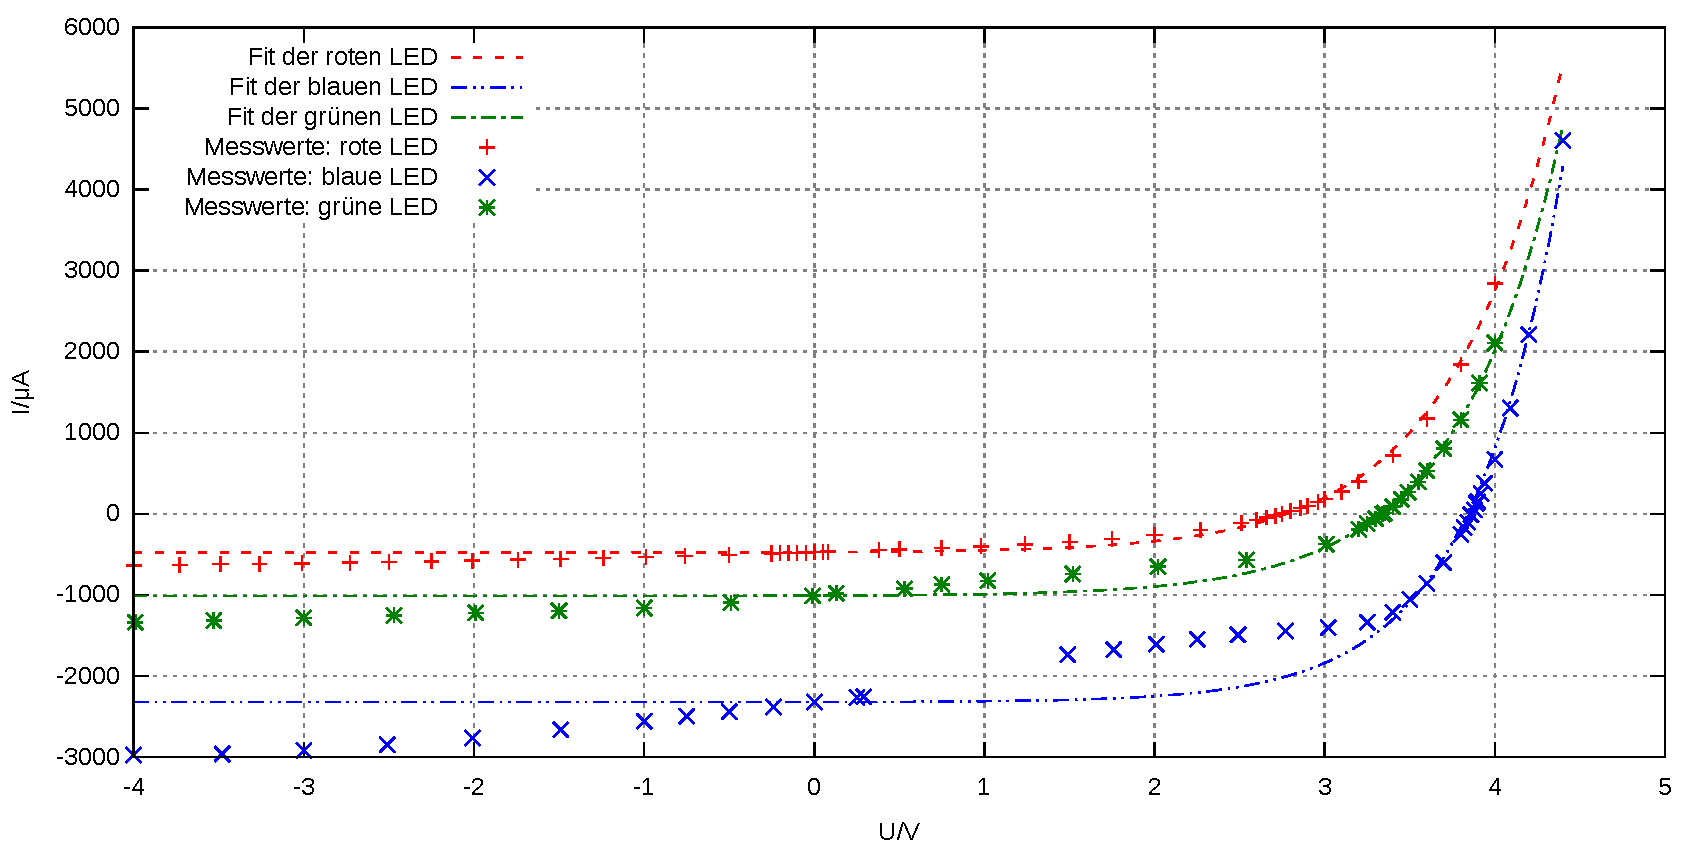
\includegraphics[width=1\textwidth]{messwerte/stromspannungspannungsrichtigled.pdf}
	\vspace{-2em}
	\caption{Diagramm: Beleuchtung mit LEDs} \label{img:ssrl}
\end{figure}
Nach dieser Messung haben wir anstelle der Spannungsquelle einen ohmschen Dekadenwiderstand (eine Last) geschaltet und unter Veränderung des Widerstands den Strom und die Spannung gemessen. Diese Messwerte wurden in den Tabellen \ref{tab:rotb} und \ref{tab:blaub} zusammengetragen und in \ref{img:ssrbl} veranschaulicht und wie zuvor an eine Funktion angepasst. Man sieht bereits im Diagramm die starke Abweichung der Messwerte der roten LED von der angepassten Kurve, was sich auch in den Fit-Parametern ausdrückt, die Größenordnungen von den übrigen Werten entfernt sind. Diese Messung wird demnach in den folgenden Betrachtungen nur der Vollständigkeit halber mit aufgeführt, aber ansonsten ignoriert.
\begin{figure}[H]
	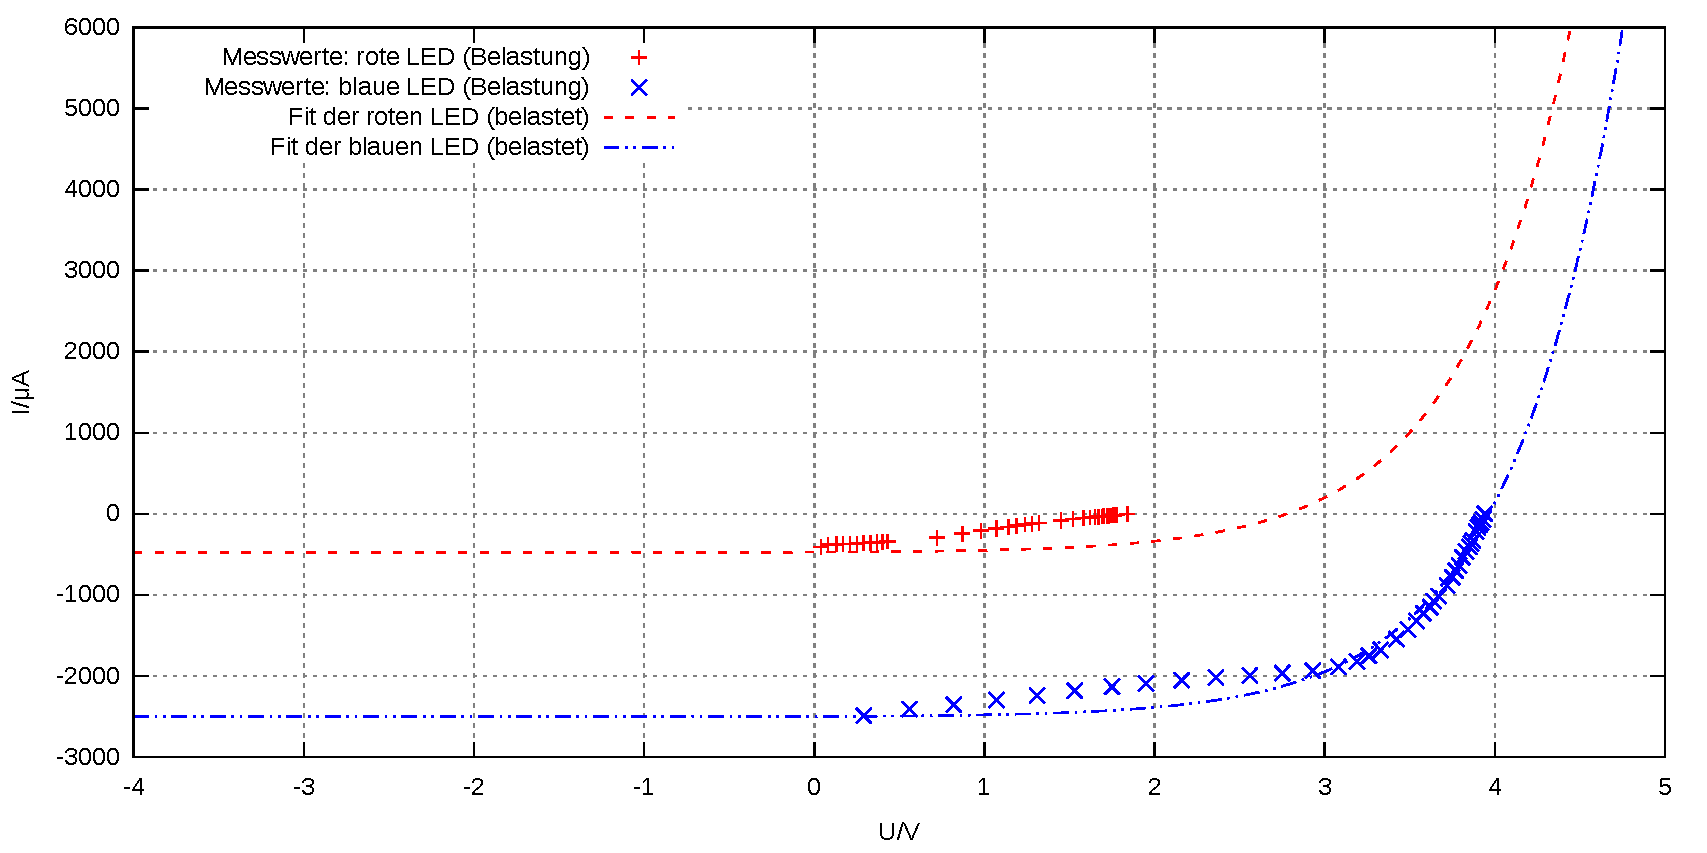
\includegraphics[width=1\textwidth]{messwerte/stromspannungspannungsrichtigbelastungled.pdf}
	\vspace{-2em}
	\caption{Diagramm: LEDs unter Belastung} \label{img:ssrbl}
\end{figure}
Gleiches wurde bei Beleuchtung durch eine starke Glühlampe und unter Sonneinstrahlung getan, die Messwerte dazu finden sich in \ref{tab:lampe} bis \ref{tab:sonne} und das zugehörige Diagramm ist \ref{img:sslus}.
\begin{figure}[H]
	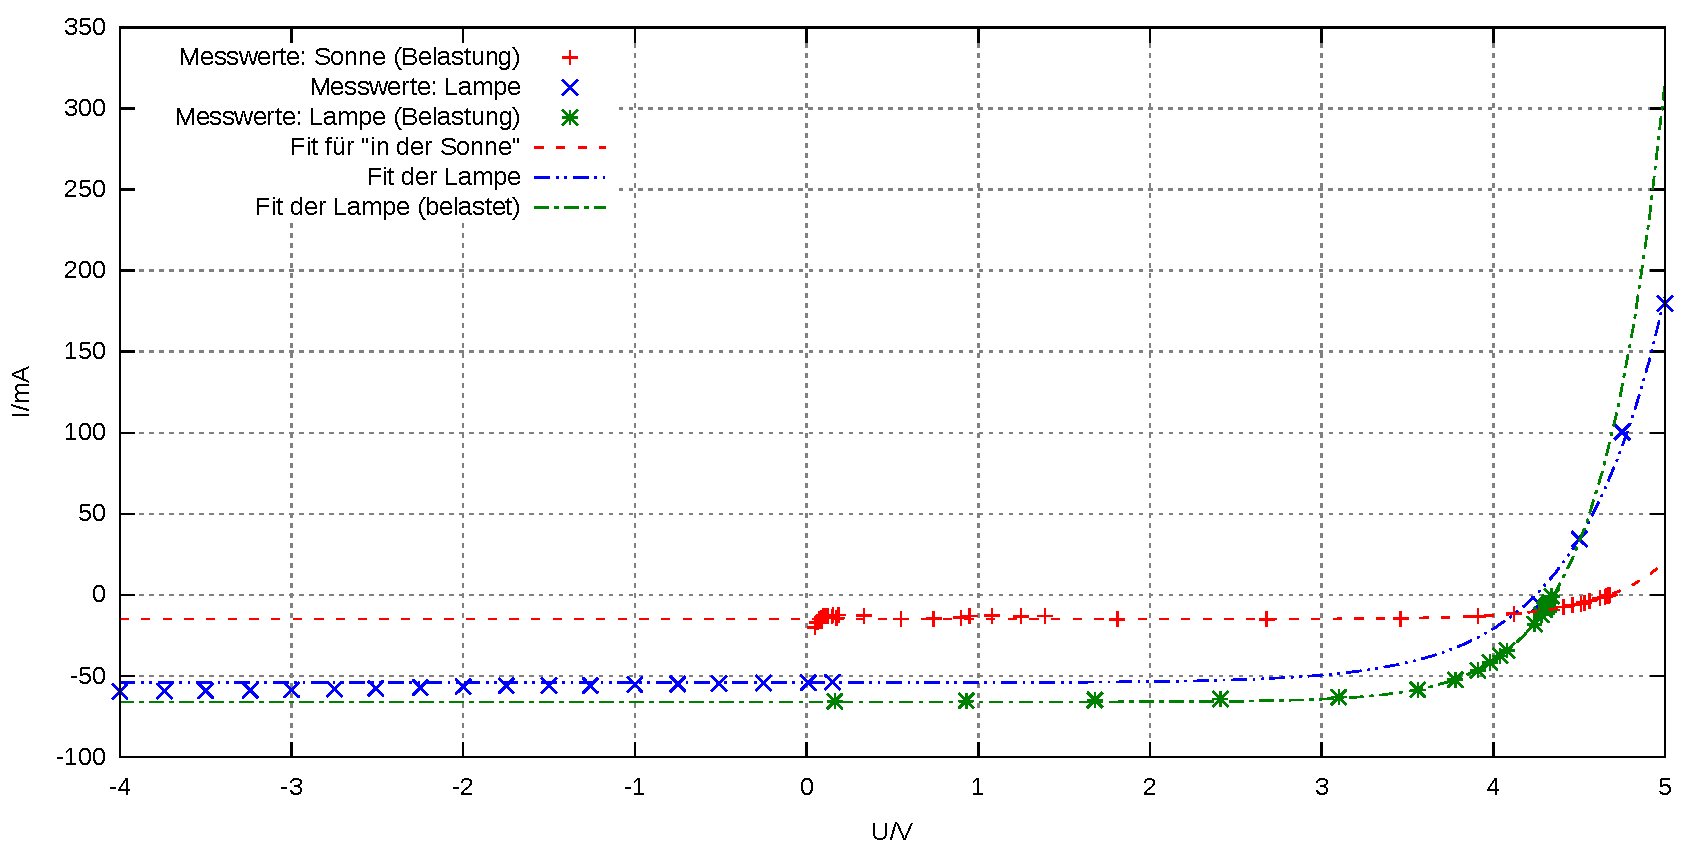
\includegraphics[width=1\textwidth]{messwerte/stromspannunglampeundsonne.pdf}
	\vspace{-2em}
	\caption{Diagramm: Sonne und Lampe} \label{img:sslus}
	\vspace{-1em}
\end{figure}
Durch den Vergleich der Beziehungen über Fotostrom und den Strom durch die Solarzelle mit den Strom-Spannungs-Charakteristiken fällt sofort auf, dass $\eta\ix{opt}$ stark von $\lambda$, also der Art der Beleuchtung, abhängen muss. $I\ix{F}$ wächst bei fallender Wellenlänge an. Weiterhin beeinträchtigen Schwankungen in der Temperatur die Güte der Messung. Besonders in \ref{img:ssrl} ist die Diskrepanz zwischen exponentieller Form und der gemessenen Kurve im dritten Quadranten gut zu erkennen. Dort könnte der Strom eine Erwärmung und damit eine in Gleichung (\ref{eq:IUenhanced}) nich berücksichtigte Schwankung der Parameter hervorgerufen haben.\\
Entgegen der Theorie, in welcher die Charakteristiken von belasteter und unbelasteter Solarzelle für gleiche Beleuchtungen zusammenfallen, konnte kein solches Verhalten unmittelbar beobachtet werden. Jedoch finden wir bemerkenswert, dass fast alle Datensätze (bis auf die bereits genannte Ausnahme) Fit-Parameter in ungefähr der selben Größenordnung liefern. Die Messungen mit der blauen LED und der Lampe haben in den charakteristischen Faktoren (Tabelle \ref{tab:faktoren}) sogar eine recht gute Übereinstimmung.\\
Die maximal nutzbare Leistung haben wir durch die Ableitung der Leistung $P=I\cdot U$ nach der Spannung festgestellt. Dafür haben wir die in den Fits erhaltenen Funktionen $I(U)$ benutzt. Da die analytische Lösung der Gleichung $\frac{\diff P}{\diff U}=0$ sich als schwierig erweist und bei unserer Messgenauigkeit auch keinen Vorteil gegenüber einer grafischen Lösungsmethode bringt, haben wir die Funktion $\frac{\diff P}{\diff U}$ in einem kleinen Bereich um $\unit[0]{A}$ aufgetragen und den Nulldurchgang abgelesen, wie in \ref{img:maxleistung} zu sehen ist (die beinahe senkrechten Linien kommen durch den kleinen Wertebereich zustande). Diese Spannung konnten wir nun wiederum in $I(U)\cdot U$ einsetzen, um die maximale Leistung zu berechnen -- die Ergebnisse sind auch in Tabelle \ref{tab:fits} eingetragen. Sowohl die Nulldurchgänge der Leistungsableitung, als auch die daraus berechneten Maximalleistungen, liegen bei den unter Last und mit der Spannungsquelle vorgenommenen Messungen dicht beieinander.
\begin{figure}[H]
	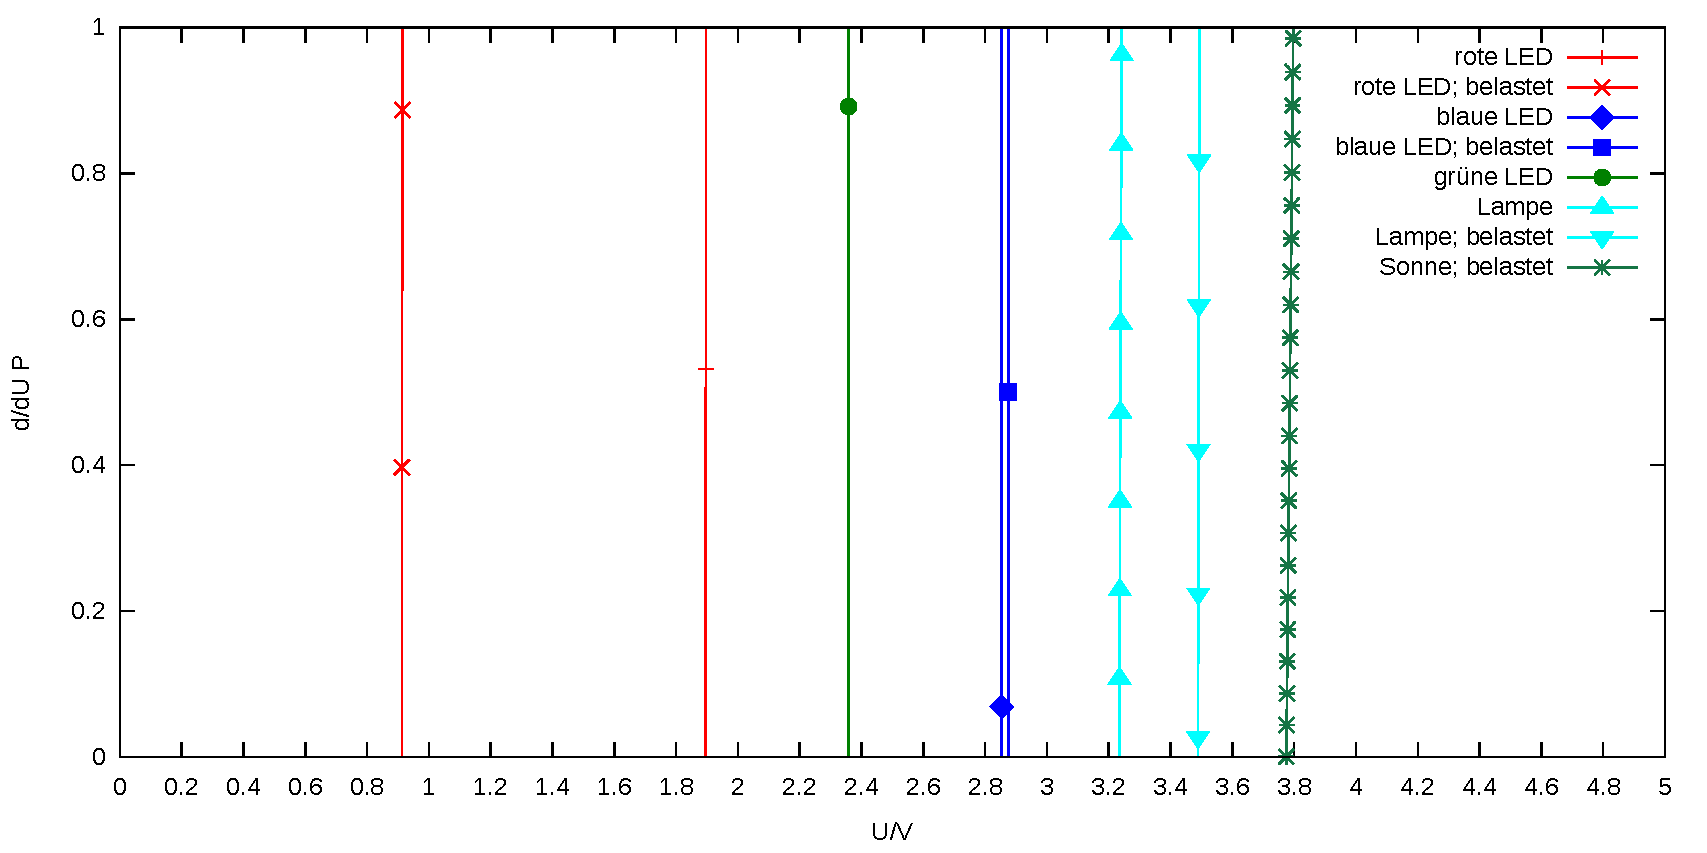
\includegraphics[width=\textwidth]{messwerte/leistungsmaxima.pdf}
	\caption{Ableitung der abgegriffenen Leistung über Spannung in einem kleinen Wertebereich}
	\label{img:maxleistung}
\end{figure}
\begin{table}[H]
	\begin{align*}
	\begin{array}{c|c|c|c|c|c}
		\text{Bedingungen} & \unit[I\ix{S}]{/\text{\greek{μ}}A} & \unit[U\ix{T}^{-1}]{/V^{-1}}  & \unit[I\ix{F}]{/\text{\greek{µ}}A} & \unit[U\ix{L}]{/V} & \unit[P\ix{max}]{/\text{\greek{µ}}W} \\ \hline
		\text{rote LED} & 6,281 & 1,560 & 473,0 & 2,777 & -412,491 \\
		\text{blaue LED} & 1,770 & 1,869 & 2322,0 & 3,841 & -5584,089 \\
		\text{grüne LED} & 4,544 & 1,625 & 1009,0 & 3,327 & -1895,289 \\
		\text{rot; belastet} & 1,0814\tenpo{4} & 0,021 & 440,0 & 1,815 & 39,619 \\
		\text{blau; belastet} & 5,221 & 1,556 & 2500,0 & 3,966 & -5885,519 \\
		\text{Lampe} & 12,6 & 1,968 & 5,41\tenpo{4} & 4,248 & -1,512\tenpo{5} \\
		\text{Lampe; belastet} & 0,485 & 2,715 & 6,6\tenpo{4} & 4,353 & -2,082\tenpo{5} \\
		\text{Sonne; belastet} & 6,18\tenpo{-2} & 2,649 & 1,5\tenpo{4} & 4,679 & -5,147\tenpo{4} \\
	\end{array}
	\end{align*}
	\caption{Fitparameter und maximale Leistung für \ref{img:ssrl} bis \ref{img:sslus}} \label{tab:fits}
\end{table}
\begin{table}[H]
	\begin{align*}
		\begin{array}{c|c|c|c}
		\text{Bedingungen} & FF & SF & CF \\ \hline
		\text{rote LED} & -0,3139 & 2,479 & -0,778 \\
		\text{blaue LED} & -0,626 & 3,429 & -2,147 \\
		\text{grüne LED} & -0,564 & 2,970 & -1,677 \\
		\text{rot; belastet} &  0,0495 & 1,621 & 0,08039 \\
		\text{blau; belastet} & -0,593 & 3,541 & -2,101 \\
		\text{Lampe} & -0,657 & 3,793 & -2,495 \\
		\text{Lampe; belastet} & -0,724 & 3,887 & -2,817 \\
		\text{Sonne; belastet} & -0,733 & 4,178 & -3,063 \\
		\end{array}
	\end{align*}
	\caption{Charakteristische Faktoren der Solarzelle} \label{tab:faktoren}
\end{table}

\section{Anhang}
\subsection{Messwerte}
\begin{table}[H]
	\begin{align*}
\begin{array}{c|c}
\unit[U]{/V} & \unit[I]{/\text{\greek{µ}}A}\\\hline
	-4,00 & -636 \\
	-3,73 & -629 \\
	-3,49 & -622 \\
	-3,26 & -617 \\
	-3,01 & -610 \\
	-2,73 & -602 \\
	-2,50 & -596 \\
	-2,25 & -586 \\
	-2,01 & -576 \\
	-1,74 & -566 \\
	-1,49 & -557 \\
	-1,24 & -545 \\
	\end{array}
	\hspace{2em}
	\begin{array}{c|c}
	\unit[U]{/V} & \unit[I]{/\text{\greek{µ}}A}\\\hline
	-0,99 & -533 \\
	-0,76 & -521 \\
	-0,50 & -506 \\
	-0,25 & -490 \\
	-0,20 & -486 \\
	-0,15 & -484 \\
	-0,10 & -481 \\
	-0,05 & -478 \\
	0,00 & -473 \\
	0,05 & -470 \\
	0,08 & -467 \\
	0,38 & -446 \\
	\end{array}
	\hspace{2em}
	\begin{array}{c|c}
	\unit[U]{/V} & \unit[I]{/\text{\greek{µ}}A}\\\hline
	0,50 & -438 \\
	0,75 & -420 \\
	0,98 & -401 \\
	1,24 & -377 \\
	1,50 & -347 \\
	1,75 & -311 \\
	2,00 & -263 \\
	2,27 & -198 \\
	2,51 & -116 \\
	2,60 & -77 \\
	2,66 & -46 \\
	2,71 & -22 \\
	\end{array}
	\hspace{2em}
	\begin{array}{c|c}
	\unit[U]{/V} & \unit[I]{/\text{\greek{µ}}A}\\\hline
	2,75 & 2 \\
	2,80 & 34 \\
	2,86 & 70 \\
	2,90 & 99 \\
	2,96 & 143 \\
	3,00 & 182 \\
	3,10 & 273 \\
	3,20 & 398 \\
	3,40 & 719 \\
	3,60 & 1175 \\
	3,80 & 1843 \\
	4,00 & 2842
\end{array}  
\end{align*}
\vspace{-1em}
\caption{Messwerte bei Beleuchtung mit der roten LED}
\label{tab:rot}
\end{table}


\begin{table}[H]
	\begin{align*}
	\begin{array}{c|c|c}
	\unit[U]{/V} & \unit[I]{/\text{\greek{µ}}A} & \unit[R]{/k\text{\greek{Ω}}}\\\hline
	0,04 & -412 & 0 \\
	0,08 & -380 & 0,1 \\
	0,13 & -376 & 0,2 \\
	0,17 & -373 & 0,3 \\
	0,21 & -370 & 0,4 \\
	0,25 & -366 & 0,5 \\
	0,29 & -360 & 0,6 \\
	0,33 & -356 & 0,7 \\
	0,37 & -351 & 0,8 \\
	0,40 & -347 & 0,9 \\
	0,43 & -341 & 1, \\
	0,72 & -294 & 2, \\
	\end{array}
	\hspace{2em}
	\begin{array}{c|c|c}
	\unit[U]{/V} & \unit[I]{/\text{\greek{µ}}A} & \unit[R]{/k\text{\greek{Ω}}}\\\hline
	0,87 & -244 & 3, \\
	0,98 & -207 & 4, \\
	1,07 & -180 & 5, \\
	1,14 & -160 & 6, \\
	1,19 & -145 & 7, \\
	1,24 & -132 & 8, \\
	1,28 & -121 & 9, \\
	1,32 & -112 & 10, \\
	1,45 & -82,4 & 15, \\
	1,52 & -65,3 & 20, \\
	1,58 & -54,2 & 25, \\
	1,62 & -46,2 & 30, \\
	\end{array}
	\hspace{2em}
	\begin{array}{c|c|c}
	\unit[U]{/V} & \unit[I]{/\text{\greek{µ}}A} & \unit[R]{/k\text{\greek{Ω}}}\\\hline
	1,65 & -40,4 & 35, \\
	1,67 & -35,8 & 40, \\
	1,69 & -32,2 & 45 \\
	1,70 & -29,2 & 50, \\
	1,72 & -26,8 & 55, \\
	1,73 & -24,6 & 60, \\
	1,74 & -21,3 & 70, \\
	1,76 & -18,8 & 80, \\
	1,77 & -16,8 & 90, \\
	1,78 & -15,2 & 100, \\
	1,84 & 0,00 & \approx\infty \\		
	\, & \, & \,
	\end{array}  
	\end{align*}
	\vspace{-1em}
	\caption{Messwerte bei Beleuchtung mit der roten LED unter angegebener Belastung}
	\label{tab:rotb}
\end{table}
\begin{table}[H]
	\begin{align*}
	\begin{array}{c|c}
	\unit[U]{/V} & \unit[I]{/\text{\greek{µ}}A}\\\hline
	-4,00 & -2976 \\
	-3,48 & -2962 \\
	-3,00 & -2919 \\
	-2,51 & -2850 \\
	-2,01 & -2766 \\
	-1,49 & -2663 \\
	-1,00 & -2557 \\
	-0,75 & -2498 \\
	-0,50 & -2442 \\
	-0,24 & -2383 \\
	\end{array}
	\hspace{2em}
	\begin{array}{c|c}
	\unit[U]{/V} & \unit[I]{/\text{\greek{µ}}A}\\\hline
	0,00 & -2322 \\
	0,25 & -2266 \\
	0,29 & -2255 \\
	1,49 & -1738 \\
	1,76 & -1673 \\
	2,01 & -1607 \\
	2,25 & -1547 \\
	2,49 & -1492 \\
	2,77 & -1445 \\
	3,02 & -1404 \\
	\end{array}
	\hspace{2em}
	\begin{array}{c|c}
	\unit[U]{/V} & \unit[I]{/\text{\greek{µ}}A}\\\hline
	3,25 & -1337 \\
	3,40 & -1213 \\
	3,50 & -1054 \\
	3,60 & -857 \\
	3,70 & -603 \\
	3,80 & -257 \\
	3,82 & -171 \\
	3,84 & -105 \\
	3,86 & -11,6 \\
	3,88 & 50 \\
	\end{array}
	\hspace{2em}
	\begin{array}{c|c}
	\unit[U]{/V} & \unit[I]{/\text{\greek{µ}}A}\\\hline
	3,89 & 126,3 \\
	3,90 & 149 \\
	3,92 & 250 \\
	3,94 & 377 \\
	4,00 & 672 \\
	4,09 & 1306 \\
	4,20 & 2211 \\
	4,40 & 4608 \\
	\, & \, \\
	\, & \, \\
	\end{array}  
\end{align*}
\vspace{-1em}
\caption{Messwerte bei Beleuchtung mit der blauen LED}
\label{tab:blau}
\end{table}

\begin{table}[H]
	\begin{align*}
	\begin{array}{c|c|c}
	\unit[U]{/V} & \unit[I]{/\text{\greek{µ}}A} & \unit[R]{/k\text{\greek{Ω}}}\\\hline
0,29 & -2490 & 0 \\
0,56 & -2410 & 0,1 \\
0,82 & -2356 & 0,2 \\
1,07 & -2297 & 0,3 \\
1,31 & -2242 & 0,4 \\
1,53 & -2181 & 0,5 \\
1,75 & -2134 & 0,6 \\
1,95 & -2091 & 0,7 \\
2,16 & -2053 & 0,8 \\
2,36 & -2020 & 0,9 \\
2,56 & -1992 & 1, \\
2,75 & -1963 & 1,1 \\
2,93 & -1935 & 1,2 \\
\end{array}
\hspace{2em}
\begin{array}{c|c|c}
\unit[U]{/V} & \unit[I]{/\text{\greek{µ}}A} & \unit[R]{/k\text{\greek{Ω}}}\\\hline
3,08 & -1888 & 1,3 \\
3,19 & -1822 & 1,4 \\
3,26 & -1751 & 1,5 \\
3,33 & -1679 & 1,6 \\
3,42 & -1545 & 1,8 \\
3,49 & -1426 & 2, \\
3,54 & -1322 & 2,2 \\
3,58 & -1230 & 2,4 \\
3,62 & -1149 & 2,6 \\
3,64 & -1078 & 2,8 \\
3,67 & -1015 & 3, \\
3,72 & -885 & 3,5 \\
3,75 & -784 & 4, \\
\end{array}
\hspace{2em}
\begin{array}{c|c|c}
\unit[U]{/V} & \unit[I]{/\text{\greek{µ}}A} & \unit[R]{/k\text{\greek{Ω}}}\\\hline
3,77 & -703 & 4,5 \\
3,79 & -637 & 5, \\
3,81 & -536,7 & 6, \\
3,83 & -463,4 & 7, \\
3,85 & -407,7 & 8, \\
3,86 & -363,8 & 9, \\
3,87 & -328,0 & 10, \\
3,89 & -220,9 & 15, \\
3,90 & -166,3 & 20, \\
3,91 & -133,5 & 25, \\
3,92 & -111,4 & 30, \\
3,93 & -67,0 & 50, \\
3,94 & 0,00 & \approx\infty \\
\end{array}
\end{align*}
\vspace{-1em}
\caption{Messwerte bei Beleuchtung mit der blauen LED unter angegebener Belastung}
\label{tab:blaub}
\end{table}

\begin{table}[H]
	\begin{align*}
	\begin{array}{c|c}
	\unit[U]{/V} & \unit[I]{/\text{\greek{µ}}A}\\\hline
-3,99 & -1338 \\
-3,53 & -1315 \\
-3,00 & -1283 \\
-2,47 & -1252 \\
-1,99 & -1222 \\
-1,50 & -1197 \\
-1,00 & -1162 \\
-0,49 & -1094 \\
\end{array}
\hspace{2em}
\begin{array}{c|c}
\unit[U]{/V} & \unit[I]{/\text{\greek{µ}}A}\\\hline
-0,01 & -1010 \\
0,13 & -980 \\
0,53 & -924 \\
0,75 & -871 \\
1,02 & -827 \\
1,52 & -742 \\
2,02 & -653 \\
2,54 & -568 \\
\end{array}
\hspace{2em}
\begin{array}{c|c}
\unit[U]{/V} & \unit[I]{/\text{\greek{µ}}A}\\\hline
3,01 & -375 \\
3,20 & -192 \\
3,25 & -122 \\
3,30 & -59 \\
3,34 & -4,2 \\
3,35 & 11,3 \\
3,40 & 87,5 \\
3,45 & 179 \\
\end{array}
\hspace{2em}
\begin{array}{c|c}
\unit[U]{/V} & \unit[I]{/\text{\greek{µ}}A}\\\hline
3,49 & 267 \\
3,55 & 394 \\
3,60 & 531 \\
3,70 & 804 \\
3,80 & 1159 \\
3,91 & 1614 \\
4,00 & 2107 \\
\, & \,
	\end{array}  
	\end{align*}
	\vspace{-1em}
	\caption{Messwerte bei Beleuchtung mit der grünen LED}
	\label{tab:grun}
\end{table}

\begin{table}[H]
	\begin{align*}
	\begin{array}{c|c}
	\unit[U]{/V} & \unit[I]{/mA}\\\hline
	5,00 & 179,8 \\
	4,75 & 100,5 \\
	4,50 & 34,5 \\
	4,27 & -5,71 \\
	0,15 & -53,85 \\
	0,01 & -54,10 \\
	\end{array}
	\hspace{2em}
	\begin{array}{c|c}
	\unit[U]{/V} & \unit[I]{/mA}\\\hline
	-0,25 & -54,38 \\
	-0,51 & -54,66 \\
	-0,75 & -54,93 \\
	-1,00 & -55,34 \\
	-1,26 & -55,85 \\
	-1,50 & -56,00 \\
	\end{array}
	\hspace{2em}
	\begin{array}{c|c}
	\unit[U]{/V} & \unit[I]{/mA}\\\hline
	-1,75 & -56,12 \\
	-2,00 & -56,60 \\
	-2,25 & -57,08 \\
	-2,51 & -57,78 \\
	-2,75 & -58,12 \\
	-3,00 & -58,47 \\
	\end{array}
	\hspace{2em}
	\begin{array}{c|c}
	\unit[U]{/V} & \unit[I]{/mA}\\\hline
	-3,24 & -58,83 \\
	-3,50 & -59,17 \\
	-3,74 & -59,41 \\
	-4,00 & -59,51 \\
	\, & \, \\
	\, & \, \\
	\end{array}  
	\end{align*}
	\vspace{-1em}
	\caption{Messwerte bei Beleuchtung mit der Lampe}
	\vspace{-1em}
	\label{tab:lampe}
\end{table}
\begin{table}[H]
	\begin{align*}
	\begin{array}{c|c|c}
	\unit[U]{/V} & \unit[I]{/mA} & \unit[R]{/k\text{\greek{Ω}}}\\\hline
	0,165 & 65,7 & 0 \\
	0,93 & 65,4 & 0,01 \\
	1,68 & 64,8 & 0,02 \\
	2,41 & 64,2 & 0,03 \\
	3,10 & 63,1 & 0,04 \\
	3,56 & 58,6 & 0,05 \\
	\end{array}
	\hspace{2em}
	\begin{array}{c|c|c}
	\unit[U]{/V} & \unit[I]{/mA} & \unit[R]{/k\text{\greek{Ω}}}\\\hline
	3,78 & 52,28 & 0,06 \\
	3,91 & 46,52 & 0,07 \\
	3,98 & 41,69 & 0,08 \\
	4,04 & 37,62 & 0,09 \\
	4,08 & 34,34 & 0,1 \\
	4,24 & 18,04 & 0,2 \\
	\end{array}
	\hspace{2em}
	\begin{array}{c|c|c}
	\unit[U]{/V} & \unit[I]{/mA} & \unit[R]{/k\text{\greek{Ω}}}\\\hline
	4,28 & 12,15 & 0,3 \\
	4,30 & 9,20 & 0,4 \\
	4,31 & 7,38 & 0,5 \\
	4,32 & 6,16 & 0,6 \\
	4,33 & 4,63 & 0,8 \\
	4,34 & 0,91 & 4 \\
	\end{array}
	\end{align*}
	\vspace{-1em}
	\caption{Messwerte bei Beleuchtung mit der Lampe unter angegebener Belastung}
	\vspace{-1em}
	\label{tab:lampeb}
\end{table}
\begin{table}[H]
	\begin{align*}
	\begin{array}{c|c|c}
	\unit[U]{/V} & \unit[I]{/\text{\greek{µ}}A} & \unit[R]{/\text{\greek{Ω}}}\\\hline
0,05 & 20,0 & 0 \\
0,063 & 17,0 & 1 \\
0,075 & 15,0 & 2 \\
0,088 & 14,0 & 3 \\
0,098 & 13,2 & 4 \\
0,111 & 12,9 & 5 \\
0,126 & 12,8 & 6 \\
0,147 & 13,3 & 7 \\
0,154 & 12,5 & 8 \\
0,174 & 14,3 & 9 \\
0,185 & 12,5 & 10 \\
0,335 & 12,8 & 20 \\
\end{array}
\hspace{2em}
\begin{array}{c|c|c}
\unit[U]{/V} & \unit[I]{/mA} & \unit[R]{/\text{\greek{Ω}}}\\\hline
0,55 & 14,8 & 30 \\
0,74 & 14,7 & 40 \\
0,90 & 14,0 & 50 \\
0,95 & 13,0 & 60 \\
1,08 & 12,8 & 70 \\
1,25 & 13,1 & 80 \\
1,39 & 12,9 & 90 \\
1,81 & 15,1 & 100 \\
2,68 & 15,1 & 150 \\
3,46 & 14,7 & 200 \\
3,91 & 13,1 & 250 \\
4,12 & 11,63 & 300 \\
\end{array}
\hspace{2em}
\begin{array}{c|c|c}
\unit[U]{/V} & \unit[I]{/mA} & \unit[R]{/\text{\greek{Ω}}}\\\hline
4,27 & 10,32 & 350 \\
4,34 & 9,21 & 400 \\
4,41 & 7,47 & 500 \\
4,46 & 6,32 & 600 \\
4,51 & 5,47 & 700 \\
4,53 & 4,81 & 800 \\
4,56 & 3,87 & 1000 \\
4,62 & 1,96 & 2000 \\
4,65 & 1,31 & 3000 \\
4,66 & 0,78 & 5000 \\
4,67 & 0,394 & 10000 \\
4,68 & 0,198 & 20000 \\
\end{array}
\end{align*}
\vspace{-1em}
\caption{Messwerte "`in der Sonne"' unter angegebener Belastung}
\vspace{-1em}
\label{tab:sonne}
\end{table}
\section{Quellen}
\ref{img:Eniv}: \url{https://de.wikipedia.org/wiki/Datei:Energy_band_model_(DE).svg} (Urheber: Wikipedia-Benutzer \textsc{Cepheiden})\\
\url{https://de.wikipedia.org/wiki/Solarzelle}\\
\url{https://de.wikipedia.org/wiki/Halbleiter}\\
Versuchsanleitung "`Solarzellen"'
\end{document}